\section{BackPropagation}\label{backpropagation}

\subsection{Algorithm}\label{algorithm}

\subsubsection{Definitions}\label{definitions}

\begin{itemize}
\tightlist
\item
  K = number of output units\\
\item
  L = number of layers in network\\
\item
  \(s_{l} =\) number of units in layer l
\item
  m = number of training examples
\item
  E - another symbol for cost function J
\end{itemize}

\subsubsection{Steps}\label{steps}

\begin{enumerate}
\def\labelenumi{\arabic{enumi}.}
\tightlist
\item
  Perform Forward Propagation -\textgreater{} Result is going be in the
  size of (m * K )
\end{enumerate}

Example of forward propagation\\
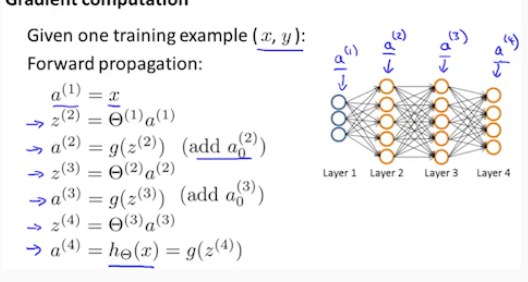
\includegraphics{forwardProp.png}

\begin{enumerate}
\def\labelenumi{\arabic{enumi}.}
\setcounter{enumi}{1}
\tightlist
\item
  Calculate the cost

  \begin{itemize}
  \tightlist
  \item
    Definitions

    \begin{itemize}
    \tightlist
    \item
      \(\theta\) - Hypothesis function parameters
    \item
      \(h_{\theta}()_ {k}\) Hypothesis function
    \item
      \(x^{(i)}\) i-th training data
    \end{itemize}
  \item
    \(\begin{gather*} J(\Theta) = - \frac{1}{m} \sum_{i=1}^m \sum_{k=1}^K \left[y^{(i)}_k \log ((h_\Theta (x^{(i)}))_ k) + (1 - y^{(i)}_k)\log (1 - (h_\Theta(x^{(i)}))_ k)\right] + \frac{\lambda}{2m}\sum_ {l=1}^{L-1} \sum_{i=1}^{s_l} \sum_{j=1}^{s_{l+1}} ( \Theta_{j,i}^{(l)})^2\end{gather*}\)
  \end{itemize}
\item
  Calculate derivatives of Cost Function according to every
  \(z^{l}_{s}\) \(\frac{\partial E}{\partial z^{l}_{s}}\)\\
\item
  Calculate derivatives for every theta
\end{enumerate}

\subsection{Derivatives}\label{derivatives}

\subsubsection{\texorpdfstring{3. Step - Calculating
\(\frac{\partial E}{\partial z^{l}_{s}} = \delta^{l}\)}{3. Step - Calculating \textbackslash{}frac\{\textbackslash{}partial E\}\{\textbackslash{}partial z\^{}\{l\}\_\{s\}\} = \textbackslash{}delta\^{}\{l\}}}\label{step---calculating-fracpartial-epartial-zl_s-deltal}

\paragraph{\texorpdfstring{1 Calculating
\(\frac{\partial E}{\partial z{L-2}} = \delta^{L}\)}{1 Calculating \textbackslash{}frac\{\textbackslash{}partial E\}\{\textbackslash{}partial z\{L-2\}\} = \textbackslash{}delta\^{}\{L\}}}\label{calculating-fracpartial-epartial-zl-2-deltal}

It is important to note that \(\delta\) is pretty much
\(\frac{\partial E}{\partial z}\) for all z.\\
Calculating \(\delta^{L}\) is different from calculating
\(\delta^{L-1}\) \(\delta^{L-2}\) \ldots{} \(\delta^{2}\)

\begin{enumerate}
\def\labelenumi{\arabic{enumi}.}
\item
  You have to calculate \(\frac{\partial E}{\partial a}\)
\item
  Then you have to calculate
  \(\frac{\partial E}{\partial a^{L}} = \frac{y}{a^{L}}+\frac{(1-y)}{(1-a^{L})}\)
  and
  \(\frac{\partial a}{\partial z^{L}}=(a*(1-a))=\sigma(z)(1-\sigma(z))\)
  \_

  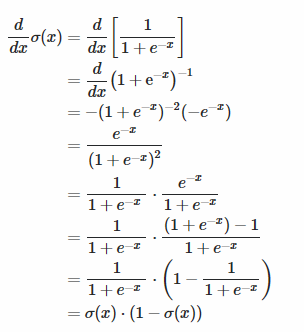
\includegraphics{sigmoidDerivative.png}

  \_
\item
  \(\frac{\partial E}{\partial z^{L}}=\frac{\partial E}{\partial a^{L}}* \frac{\partial a^{L}}{\partial z^{L}}= \delta^{(L)} = a^{L}* (1-a^{L})* (\frac{y}{a^{L}}+\frac{(1-y)}{(1-a^{L})})=a^{(L)} - y\)
\end{enumerate}

\paragraph{\texorpdfstring{2 Calculating
\(\frac{\partial E}{\partial z^{L-1}}=\delta^{(L-1)}, \frac{\partial E}{\partial z^{L-2}}=\delta^{(L-2)},\dots, \frac{\partial E}{\partial z^{L-2}}=\delta^{(2)}\)
GENERAL
CASE}{2 Calculating \textbackslash{}frac\{\textbackslash{}partial E\}\{\textbackslash{}partial z\^{}\{L-1\}\}=\textbackslash{}delta\^{}\{(L-1)\}, \textbackslash{}frac\{\textbackslash{}partial E\}\{\textbackslash{}partial z\^{}\{L-2\}\}=\textbackslash{}delta\^{}\{(L-2)\},\textbackslash{}dots, \textbackslash{}frac\{\textbackslash{}partial E\}\{\textbackslash{}partial z\^{}\{L-2\}\}=\textbackslash{}delta\^{}\{(2)\} GENERAL CASE}}\label{calculating-fracpartial-epartial-zl-1deltal-1-fracpartial-epartial-zl-2deltal-2dots-fracpartial-epartial-zl-2delta2-general-case}

\textbf{Reminder: In each level l derivative we can have multiple
\(\delta^{l}\), like we have multiple \(z^{l}\)}

Calculation is done somewhat recursively. For every smaller level
\(\delta^{l}\) we need to use \(\delta^{l+1}\) in our calculation of the
derivative because of the chain derivative rule:
\(\frac{d}{{dx}}\left[ {f\left( u \right)} \right] = \frac{d}{{du}}\left[ {f\left( u \right)} \right]\frac{{du}}{{dx}}\)
. If, inside the formula we go further from the output towards the input
we need to always take functions in between under consideration.

\textbf{In other words}

\(\frac{\partial E}{z^{l}}=\frac{\partial E}{z^{l+1}}\)
\textbf{\(\frac{\partial z^{l+1}}{ a^{l}} \frac{\partial a^{l}}{z^{l}}\)}

\textbf{This translates to}

\(\frac{\partial E}{\partial Z^{l}} = \delta^{(l)} =\)
\(((\Theta^{(l)})^T \delta^{(l+1)})\)
\(\ .* \ a^{(l)}\ .* \ (1 - a^{(l)})\)

\textbf{Where each part stands for}\\
+
\(((\Theta^{(l)})^T \delta^{(l+1)})=\frac{\partial z^{l+1}}{\partial a^{l}}\)
+ This rule is somewhat more interesting, because it applies a somewhat
complicated concept where 1 variable in a function affects the end
result through multiple other functions. E.g \(E=E(d(x),u(x))\) Such a
function, when taking a derivative is solved by just summing up all the
derivatives. \textbf{This is somewhat intuitive but I wont go to deep
into it}\\
+ Explanation in Estonian\\
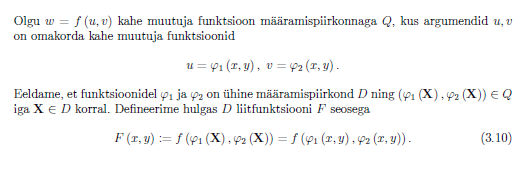
\includegraphics{matAnal1.png}\\
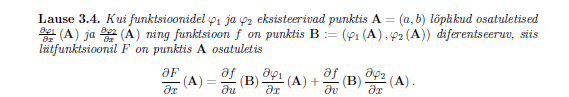
\includegraphics{matAnal2.png} +
\(\ a^{(l)}\ .* \ (1 - a^{(l)}) = \frac{\partial a^{l}}{z^{l}}\)

\subsubsection{\texorpdfstring{4. Step - Calculating
\(\frac{\partial E}{\partial \theta^{l}}\)}{4. Step - Calculating \textbackslash{}frac\{\textbackslash{}partial E\}\{\textbackslash{}partial \textbackslash{}theta\^{}\{l\}\}}}\label{step---calculating-fracpartial-epartial-thetal}

\(\frac{\partial E}{\partial \theta^{l}_{ij}}=\frac{\partial E}{z^{l+1}_{i}} \frac{\partial z^{l+1}_{i}}{\partial \theta^{l}_{ij}}\)

\textbf{This in regular derivative form translates to}

\(\frac{\partial E}{\partial \theta^{l}_{ij}}=\delta^{l+1}_{i}a^{l}_{j}\)

\textbf{This translates in vectorial form to}

\subsection{How to Check whether Gradient is
correct.}\label{how-to-check-whether-gradient-is-correct.}
